\documentclass[12pt]{article}
\usepackage[utf8]{inputenc}
\usepackage[T1]{fontenc}
\usepackage{geometry}
\geometry{margin=1in}
\usepackage{hyperref}
\usepackage{tikz}
\usepackage{pgfplots}
\usepackage{algorithm}
\usepackage{algpseudocode}
\usepackage{amsmath}
\usepackage{amssymb}
\usepackage{graphicx}
\usepackage{listings}
\usepackage{xcolor}
\usepackage{float}
\usepackage{tabularx}
\usetikzlibrary{shapes,arrows,positioning,calc,backgrounds,fit}
\pgfplotsset{compat=1.18}
\title{Sistema Distribuido Master-Slave con Ubicación Semántica}
\author{Abel Ponce González C411\\Richard Alejandro Matos Arderí C411}
\date{\today}

\begin{document}

\maketitle

\begin{abstract}
Este documento presenta la especificación arquitectónica de un sistema distribuido de búsqueda de documentos basado en arquitectura Master-Slave con elección dinámica de líder. Se detalla la arquitectura del sistema, la organización y roles de sus componentes, los mecanismos de ubicación de recursos mediante vectorización semántica, las estrategias de tolerancia a fallos con algoritmo Bully para elección de líder, el sistema de replicación por afinidad semántica, y los aspectos de seguridad y comunicación del diseño.
\end{abstract}

\tableofcontents

\newpage

\section{Introducción}

\subsection{Descripción del sistema}
El sistema propuesto es una plataforma distribuida para almacenamiento y búsqueda de documentos utilizando una arquitectura Master-Slave con elección dinámica de líder. El sistema emplea vectorización semántica para ubicación de recursos, lo que permite localizar documentos basándose en similitud de contenido en lugar de funciones hash. Esta aproximación proporciona búsquedas más relevantes y una distribución de datos más inteligente basada en afinidad de contenido.

\subsection{Objetivos del diseño}
\begin{itemize}
  \item Proporcionar alta disponibilidad mediante elección automática de líder ante fallos del Master
  \item Garantizar redundancia de datos mediante replicación basada en afinidad semántica
  \item Proporcionar mecanismos eficientes de localización de recursos mediante vectorización semántica
  \item Implementar tolerancia a fallos con detección mediante heartbeats y recuperación automática
  \item Distribuir carga entre Slaves mediante balanceo basado en carga y afinidad de contenido
  \item Permitir acceso distribuido mediante DNS con múltiples puntos de entrada
\end{itemize}

\section{Arquitectura del Sistema}

\subsection{Estilos arquitectónicos}

Según Tanenbaum \& Van Steen (2017), los sistemas distribuidos pueden clasificarse según diferentes estilos arquitectónicos. DistriSearch combina múltiples estilos para lograr sus objetivos:

\subsubsection{Arquitectura en Capas (Layered Architecture)}

El sistema implementa una \textbf{arquitectura en capas} donde cada capa proporciona servicios a la capa superior y consume servicios de la capa inferior:

\begin{figure}[H]
\centering
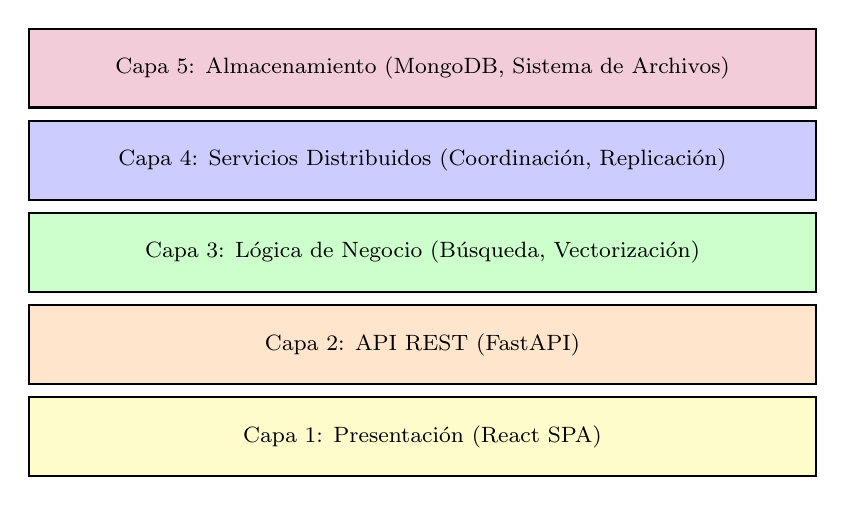
\begin{tikzpicture}[scale=0.9]
  \tikzstyle{layer}=[rectangle, draw, thick, minimum width=10cm, minimum height=1cm, font=\footnotesize]
  
  \node[layer, fill=yellow!20] (l1) at (0,0) {Capa 1: Presentación (React SPA)};
  \node[layer, fill=orange!20] (l2) at (0,1.3) {Capa 2: API REST (FastAPI)};
  \node[layer, fill=green!20] (l3) at (0,2.6) {Capa 3: Lógica de Negocio (Búsqueda, Vectorización)};
  \node[layer, fill=blue!20] (l4) at (0,3.9) {Capa 4: Servicios Distribuidos (Coordinación, Replicación)};
  \node[layer, fill=purple!20] (l5) at (0,5.2) {Capa 5: Almacenamiento (MongoDB, Sistema de Archivos)};
\end{tikzpicture}
\caption{Arquitectura en capas del sistema}
\label{fig:layered-arch}
\end{figure}

\subsubsection{Arquitectura Publish-Subscribe para Eventos}

Para la comunicación asíncrona entre componentes, el sistema utiliza el patrón \textbf{Publish-Subscribe} (Tanenbaum \& Van Steen, 2017):

\begin{itemize}
  \item \textbf{Eventos de heartbeat}: Los Slaves publican su estado; el Master y otros Slaves suscritos detectan fallos
  \item \textbf{Eventos de replicación}: Cuando se sube un documento, se publica evento para que réplicas lo reciban
  \item \textbf{Eventos de rebalanceo}: Al añadir/remover nodos, se notifica a todo el clúster
\end{itemize}

Este patrón proporciona \textbf{desacoplamiento temporal y referencial}: los publicadores no necesitan conocer a los suscriptores, y la comunicación puede ocurrir de forma asíncrona.

\subsubsection{Elementos de arquitectura Peer-to-Peer}

Aunque el sistema es principalmente Master-Slave, incorpora elementos \textbf{P2P} (Tanenbaum \& Van Steen, 2017):

\begin{itemize}
  \item \textbf{Comunicación Slave-Slave}: Los Slaves se comunican directamente para heartbeats y replicación sin pasar por el Master
  \item \textbf{Elección de líder distribuida}: Cualquier Slave puede iniciar una elección (algoritmo Bully)
  \item \textbf{Tolerancia a particiones}: Slaves en una partición de red pueden seguir operando entre sí
\end{itemize}

\subsubsection{Estilo Master-Slave con promoción dinámica}

El estilo principal es \textbf{Master-Slave} donde un nodo coordinador (Master) dirige a múltiples trabajadores (Slaves). La característica distintiva es que cualquier Slave puede convertirse en Master mediante elección cuando el Master actual falla, eliminando el punto único de fallo.

Los componentes principales son:
\begin{itemize}
  \item \textbf{Nodos Slave}: Unidades autónomas que almacenan documentos, procesan búsquedas locales y mantienen su propia instancia de MongoDB. Cada Slave incluye backend (API FastAPI) y frontend (React).
  \item \textbf{Master}: Un Slave con responsabilidades adicionales de coordinación: mantiene el índice VP-Tree global, balancea carga, coordina replicación y enruta queries.
  \item \textbf{Load Balancer}: Distribuye tráfico entrante entre Slaves disponibles (Nginx/Traefik).
\end{itemize}

\subsection{Modelo arquitectónico: Master-Slave con elección dinámica}

\subsubsection{Características del sistema}

El sistema implementa una arquitectura \textbf{Master-Slave con failover automático}. A diferencia de arquitecturas centralizadas tradicionales, el rol de Master no está fijado a un nodo específico sino que puede migrar dinámicamente entre los Slaves candidatos cuando ocurre una falla.

\textbf{Ubicación de recursos por vectorización semántica:} En lugar de utilizar funciones hash para determinar dónde almacenar documentos (como en DHT), el sistema emplea vectores TF-IDF combinados con firmas MinHash. Cada documento se representa mediante un vector TF-IDF sparse y una firma MinHash de 128 hashes que permite estimar similitud Jaccard eficientemente. El Master mantiene un índice de ubicación que mapea perfiles TF-IDF a los Slaves que contienen documentos similares, permitiendo:
\begin{itemize}
  \item Routing inteligente de queries a Slaves con contenido relevante
  \item Selección de nodos para replicación basada en afinidad de contenido
  \item Balanceo de carga considerando tanto capacidad como especialización de contenido
\end{itemize}

\begin{figure}[H]
\centering
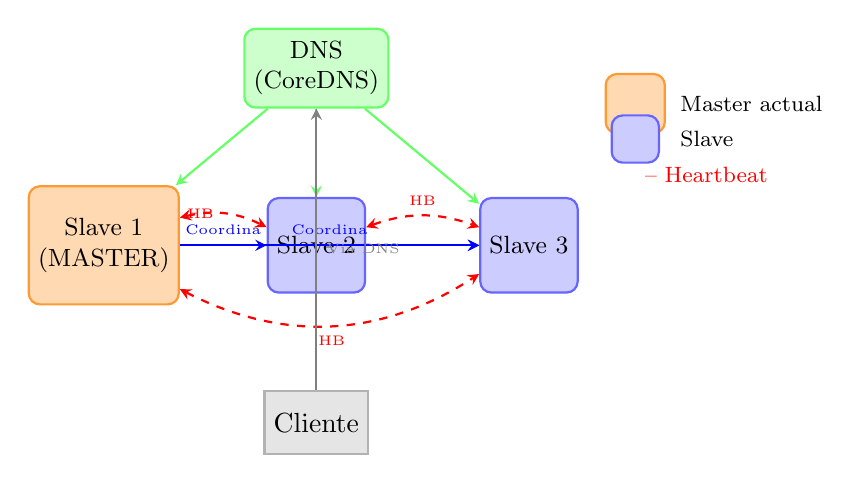
\begin{tikzpicture}[scale=0.9]
  % Definir estilos
  \tikzstyle{master}=[rectangle, draw=orange!80, fill=orange!30, thick, minimum size=1.5cm, font=\small, rounded corners, align=center]
  \tikzstyle{slave}=[rectangle, draw=blue!60, fill=blue!20, thick, minimum size=1.2cm, font=\small, rounded corners, align=center]
  \tikzstyle{dns}=[rectangle, draw=green!60, fill=green!20, thick, minimum size=1cm, font=\small, rounded corners, align=center]
  \tikzstyle{client}=[rectangle, draw=gray!60, fill=gray!20, thick, minimum size=0.8cm, align=center]
  \tikzstyle{conn}=[->, thick, >=stealth]
  \tikzstyle{heartbeat}=[<->, thick, >=stealth, red, dashed]
  
  % DNS
  \node[dns] (dns) at (3,5) {DNS \\ (CoreDNS)};
  
  % Master (actualmente Slave 1)
  \node[master] (master) at (0,2.5) {Slave 1 \\ (MASTER)};
  
  % Slaves
  \node[slave] (s2) at (3,2.5) {Slave 2};
  \node[slave] (s3) at (6,2.5) {Slave 3};
  
  % Cliente
  \node[client] (c1) at (3,0) {Cliente};
  
  % Conexiones Master-Slave
  \draw[conn, blue] (master) -- node[above, font=\tiny] {Coordina} (s2);
  \draw[conn, blue] (master) -- node[above, font=\tiny] {Coordina} (s3);
  \draw[conn, blue] (s2) -- (s3);
  
  % Heartbeats
  \draw[heartbeat] (master) to[bend left=20] node[left, font=\tiny] {HB} (s2);
  \draw[heartbeat] (s2) to[bend left=20] node[above, font=\tiny] {HB} (s3);
  \draw[heartbeat] (master) to[bend right=30] node[below, font=\tiny] {HB} (s3);
  
  % DNS resuelve a cualquier nodo
  \draw[conn, green!60] (dns) -- (master);
  \draw[conn, green!60] (dns) -- (s2);
  \draw[conn, green!60] (dns) -- (s3);
  
  % Cliente puede conectar a cualquiera via DNS
  \draw[conn, gray] (c1) -- node[right, font=\tiny] {Via DNS} (dns);
  
  % Leyenda
  \node[master, scale=0.5] at (7.5,4.5) {};
  \node[right, font=\footnotesize] at (8,4.5) {Master actual};
  \node[slave, scale=0.5] at (7.5,4) {};
  \node[right, font=\footnotesize] at (8,4) {Slave};
  \node[right, font=\footnotesize, red] at (7.5,3.5) {-- Heartbeat};
\end{tikzpicture}
\caption{Arquitectura Master-Slave: Slave 1 actúa como Master. Los heartbeats detectan fallos. DNS permite acceso a cualquier nodo.}
\label{fig:master-slave-arch}
\end{figure}

\subsection{Distribución del sistema}

\subsubsection{Distribución jerárquica Master-Slave sobre Docker Swarm}
El sistema emplea una \textbf{arquitectura Master-Slave} desplegada sobre \textbf{Docker Swarm}, el orquestador nativo de Docker que proporciona clustering, scheduling y service discovery automático. A diferencia de sistemas P2P puros, esta arquitectura proporciona un punto de coordinación centralizado que simplifica la gestión del clúster mientras mantiene la escalabilidad horizontal a través de los Slaves.

\textbf{Docker Swarm} aporta las siguientes características fundamentales (Tanenbaum \& Van Steen, 2017):
\begin{itemize}
  \item \textbf{Redes Overlay}: Comunicación multi-host mediante VXLAN, encapsulando tráfico Ethernet sobre UDP/IP
  \item \textbf{Service Discovery}: DNS interno en \texttt{127.0.0.11} que resuelve nombres de servicio a IPs virtuales
  \item \textbf{Load Balancing}: Routing mesh con IPVS para distribución de carga entre réplicas
  \item \textbf{Ingress Network}: Red overlay especial para tráfico externo con balanceo automático
\end{itemize}

Cada \textbf{Slave} es un nodo completo que integra:
\begin{itemize}
  \item \textbf{Backend}: API REST para procesamiento de consultas y gestión de documentos
  \item \textbf{Frontend}: Aplicación web React servida mediante Nginx para interacción con usuarios
  \item \textbf{Base de datos}: Instancia MongoDB local para almacenamiento de documentos
  \item \textbf{Servicios de clúster}: Heartbeat, participación en elecciones, replicación
\end{itemize}

El \textbf{Master} coordina el clúster manteniendo:
\begin{itemize}
  \item Índice semántico de ubicación de recursos
  \item Balanceador de carga entre Slaves
  \item Coordinador de replicación
  \item Enrutador de consultas
\end{itemize}

\subsection{Topología de red: Estrella con redundancia}

\subsubsection{Definición de la topología}
La red se estructura como una \textbf{topología en estrella} donde el Master actúa como nodo central y los Slaves se conectan directamente a él. Sin embargo, para garantizar tolerancia a fallos, todos los Slaves mantienen conexiones entre sí para:
\begin{itemize}
  \item \textbf{Heartbeat}: Detección de fallos mediante UDP broadcast
  \item \textbf{Elección de líder}: Algoritmo Bully para elegir nuevo Master
  \item \textbf{Replicación directa}: Sincronización de datos entre réplicas
\end{itemize}

\begin{figure}[H]
\centering
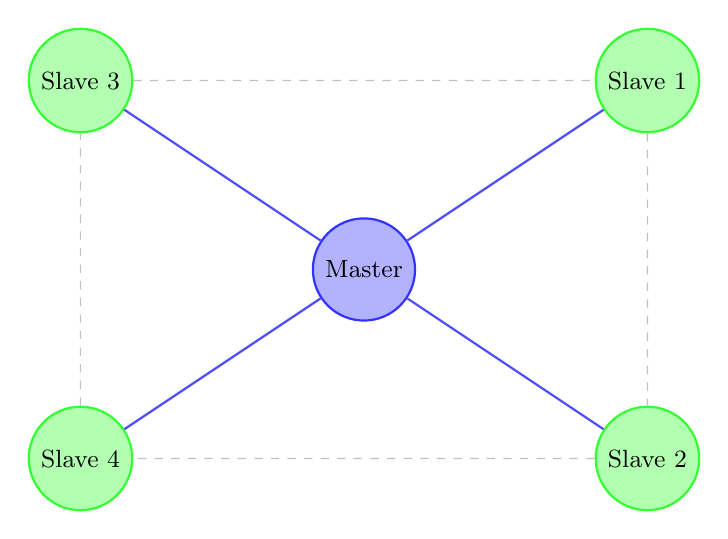
\begin{tikzpicture}[scale=1.2]
  \tikzstyle{master}=[circle, draw=blue!80, fill=blue!30, thick, minimum size=1.2cm, font=\small]
  \tikzstyle{slave}=[circle, draw=green!80, fill=green!30, thick, minimum size=1cm, font=\small]
  \tikzstyle{primary}=[-, thick, blue!70]
  \tikzstyle{secondary}=[-, dashed, gray!50]
  
  % Master en el centro
  \node[master] (m) at (0,0) {Master};
  
  % Slaves alrededor
  \node[slave] (s1) at (3,2) {Slave 1};
  \node[slave] (s2) at (3,-2) {Slave 2};
  \node[slave] (s3) at (-3,2) {Slave 3};
  \node[slave] (s4) at (-3,-2) {Slave 4};
  
  % Conexiones primarias (Master-Slave)
  \draw[primary] (m) -- (s1);
  \draw[primary] (m) -- (s2);
  \draw[primary] (m) -- (s3);
  \draw[primary] (m) -- (s4);
  
  % Conexiones secundarias (Slave-Slave para tolerancia a fallos)
  \draw[secondary] (s1) -- (s2);
  \draw[secondary] (s2) -- (s4);
  \draw[secondary] (s4) -- (s3);
  \draw[secondary] (s3) -- (s1);
\end{tikzpicture}
\caption{Topología Master-Slave: líneas sólidas = comunicación primaria, líneas punteadas = heartbeat y elección}
\label{fig:master-slave-topology}
\end{figure}

\subsubsection{Propiedades de la topología Master-Slave}
Para un clúster con \(N\) Slaves:
\begin{itemize}
  \item \textbf{Latencia de consulta}: \(O(1)\) saltos (Master enruta directamente al Slave apropiado)
  \item \textbf{Escalabilidad}: Lineal con el número de Slaves
  \item \textbf{Tolerancia a fallos}: El sistema continúa operando si falla el Master (elección automática)
  \item \textbf{Consistencia}: Eventual, con replicación configurable (factor por defecto: 2)
\end{itemize}

\textbf{Flujo de consulta típico}:
\begin{enumerate}
  \item Cliente envía consulta al Master
  \item Master calcula embeddings semánticos de la consulta
  \item Master identifica Slaves con contenido semánticamente relevante
  \item Master enruta la consulta a los Slaves seleccionados
  \item Slaves ejecutan búsqueda local y devuelven resultados
  \item Master agrega y ordena resultados finales
\end{enumerate}

\section{Roles y organización funcional}

En el sistema Master-Slave propuesto, los roles están claramente diferenciados para optimizar la coordinación y el procesamiento distribuido. El \textbf{Master} actúa como coordinador central del clúster, mientras que los \textbf{Slaves} son los nodos trabajadores que almacenan datos y procesan consultas.

El \textbf{Master} mantiene el índice semántico global de ubicación de recursos. Cuando recibe una consulta, calcula el embedding semántico y determina qué Slaves contienen información relevante. El Master no almacena documentos directamente sino metadatos sobre qué contenido tiene cada Slave.

Los \textbf{Slaves} son nodos autónomos que integran backend, frontend y base de datos. Cada Slave puede atender usuarios directamente a través de su interfaz web, procesar consultas locales y participar en la replicación de datos. Esta arquitectura permite que los Slaves operen de forma independiente incluso si el Master falla temporalmente.

Un aspecto crítico es la \textbf{elección de líder}: si el Master falla, los Slaves ejecutan el algoritmo Bully para elegir un nuevo Master entre los candidatos elegibles. Esto garantiza la continuidad del servicio sin intervención manual.

\subsection{Diagrama de roles e interacciones}

\begin{figure}[H]
\centering
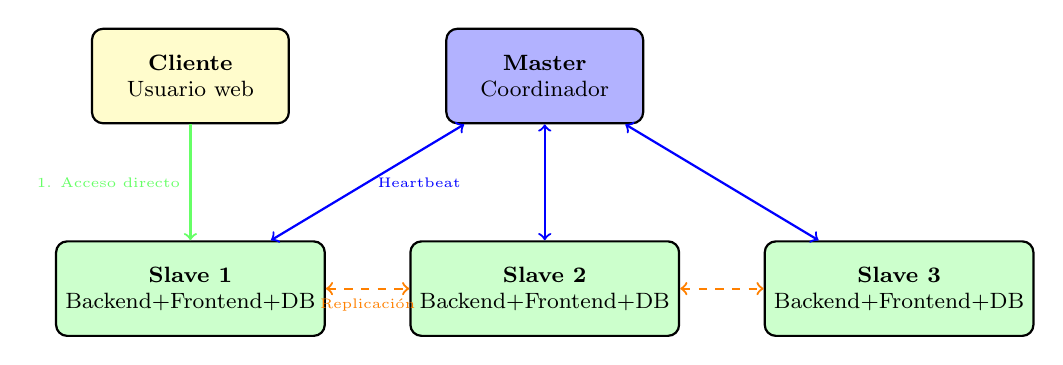
\begin{tikzpicture}[scale=0.9]
  \tikzstyle{role}=[rectangle, draw, thick, minimum width=2.5cm, minimum height=1.2cm, rounded corners, font=\footnotesize, align=center]
  \tikzstyle{master}=[role, fill=blue!30]
  \tikzstyle{slave}=[role, fill=green!20]
  \tikzstyle{client}=[role, fill=yellow!20]
  
  \node[client] (c) at (0,5) {\textbf{Cliente}\\Usuario web};
  \node[master] (m) at (5,5) {\textbf{Master}\\Coordinador};
  \node[slave] (s1) at (0,2) {\textbf{Slave 1}\\Backend+Frontend+DB};
  \node[slave] (s2) at (5,2) {\textbf{Slave 2}\\Backend+Frontend+DB};
  \node[slave] (s3) at (10,2) {\textbf{Slave 3}\\Backend+Frontend+DB};
  
  % Cliente accede a cualquier Slave
  \draw[->, thick, green!60] (c) -- node[left, font=\tiny] {1. Acceso directo} (s1);
  % Master coordina
  \draw[<->, thick, blue] (m) -- node[right, font=\tiny] {Heartbeat} (s1);
  \draw[<->, thick, blue] (m) -- (s2);
  \draw[<->, thick, blue] (m) -- (s3);
  % Replicación entre Slaves
  \draw[<->, thick, orange, dashed] (s1) -- node[below, font=\tiny] {Replicación} (s2);
  \draw[<->, thick, orange, dashed] (s2) -- (s3);
\end{tikzpicture}
\caption{Arquitectura Master-Slave: clientes acceden directamente a Slaves, Master coordina ubicación y replicación}
\label{fig:roles}
\end{figure}

\subsection{Responsabilidades de cada rol}

\begin{table}[H]
\centering
\begin{tabularx}{\textwidth}{|l|X|}
\hline
\textbf{Rol} & \textbf{Responsabilidades} \\ \hline
\textbf{Master} & 
Mantener índice semántico de ubicación de recursos, recibir registros de nuevos documentos, calcular embeddings y determinar relevancia semántica, enrutar consultas a Slaves apropiados, coordinar replicación, monitorear salud del clúster mediante heartbeats, detectar fallos de nodos. \\ \hline
\textbf{Slave} & 
Almacenar documentos en MongoDB local, servir interfaz web (frontend React con Nginx), procesar consultas de búsqueda locales, participar en elecciones de líder (algoritmo Bully), enviar heartbeats al Master, recibir y aplicar replicaciones de otros Slaves. \\ \hline
\textbf{Cliente} & 
Acceder a cualquier Slave disponible vía web, realizar búsquedas semánticas y por nombre, subir y descargar documentos, el DNS resuelve distrisearch.local a cualquier Slave saludable. \\ \hline
\end{tabularx}
\caption{Responsabilidades por rol en arquitectura Master-Slave}
\label{tab:responsibilities}
\end{table}

\section{Despliegue y distribución de servicios con Docker Swarm}

El despliegue se implementa usando \textbf{Docker Swarm} como plataforma de orquestación, aprovechando sus capacidades nativas de networking, service discovery y load balancing:

\subsection{Arquitectura de redes Docker Swarm}

\begin{description}
  \item[distrisearch-overlay] Red overlay creada con driver \texttt{overlay} que permite comunicación multi-host. Utiliza VXLAN para encapsular tráfico entre nodos físicos del Swarm.
  \item[ingress] Red overlay especial gestionada automáticamente por Swarm para tráfico externo. Implementa routing mesh con IPVS para balanceo de carga.
\end{description}

\subsubsection{Modos de endpoint para Service Discovery}
Docker Swarm ofrece dos modos de endpoint para resolución de servicios:
\begin{itemize}
  \item \textbf{VIP (Virtual IP)}: Modo por defecto. El DNS interno resuelve el nombre del servicio a una IP virtual única. El balanceador IPVS distribuye el tráfico entre réplicas.
  \item \textbf{DNSRR (DNS Round Robin)}: El DNS retorna todas las IPs de las réplicas. El cliente decide a cuál conectarse.
\end{itemize}

El sistema utiliza \textbf{VIP} para los Slaves (balanceo automático) y permite acceso directo mediante tasks individuales: \texttt{slave.1.distrisearch-overlay}, \texttt{slave.2.distrisearch-overlay}, etc.

\subsection{Comandos de despliegue con Docker Swarm}

\textbf{1. Inicializar Swarm y crear red overlay:}
\begin{verbatim}
docker swarm init --advertise-addr <IP_MANAGER>
docker network create --driver overlay \
  --attachable distrisearch-overlay
\end{verbatim}

\textbf{2. Desplegar stack con docker-compose.swarm.yml:}
\begin{verbatim}
docker stack deploy -c docker-compose.swarm.yml distrisearch
\end{verbatim}

\textbf{Configuración de servicio Master en docker-compose.swarm.yml:}
\begin{verbatim}
master:
  image: distrisearch/master:latest
  networks:
    - distrisearch-overlay
  deploy:
    replicas: 1
    placement:
      constraints: [node.role == manager]
\end{verbatim}

\textbf{3. Configuración de Slaves con MongoDB en Swarm:}
\begin{verbatim}
slave:
  image: distrisearch/slave:latest
  networks:
    - distrisearch-overlay
  environment:
    - MASTER_HOST=master  # Resuelto por DNS interno
  deploy:
    replicas: 3
    endpoint_mode: vip    # Balanceo automático
  ports:
    - target: 8000
      published: 8000
      mode: ingress       # Routing mesh

mongo:
  image: mongo:7
  networks:
    - distrisearch-overlay
  deploy:
    replicas: 3
    placement:
      max_replicas_per_node: 1
\end{verbatim}

\begin{figure}[H]
\centering
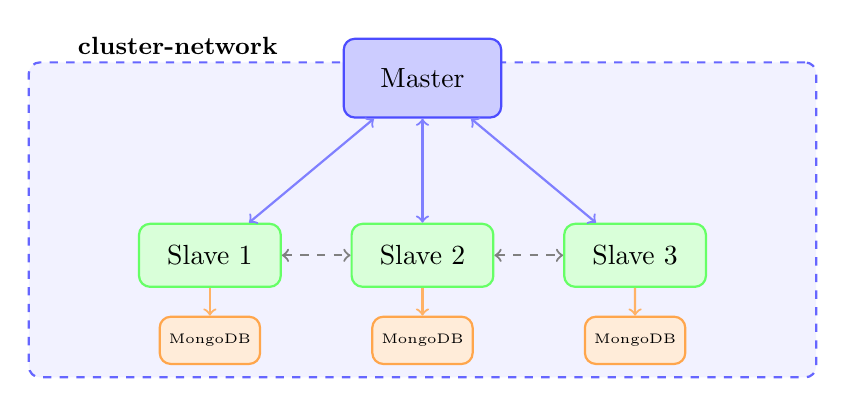
\begin{tikzpicture}[scale=0.9]
  \tikzstyle{net}=[rectangle, draw, thick, dashed, minimum width=10cm, minimum height=4cm, rounded corners]
  \tikzstyle{container}=[rectangle, draw=green!60, fill=green!15, thick, minimum width=1.8cm, minimum height=0.8cm, rounded corners]
  \tikzstyle{master}=[rectangle, draw=blue!70, fill=blue!20, thick, minimum width=2cm, minimum height=1cm, rounded corners]
  \tikzstyle{db}=[rectangle, draw=orange!70, fill=orange!15, thick, minimum width=1.2cm, minimum height=0.6cm, rounded corners]
  
  % Red del clúster
  \node[net, draw=blue!60, fill=blue!5] (cluster) at (3,2) {};
  \node[above right, font=\small] at (-2,4.2) {\textbf{cluster-network}};
  
  % Master
  \node[master] (m) at (3,4) {Master};
  
  % Slaves con MongoDB
  \node[container] (s1) at (0,1.5) {Slave 1};
  \node[db] (db1) at (0,0.3) {\tiny MongoDB};
  \node[container] (s2) at (3,1.5) {Slave 2};
  \node[db] (db2) at (3,0.3) {\tiny MongoDB};
  \node[container] (s3) at (6,1.5) {Slave 3};
  \node[db] (db3) at (6,0.3) {\tiny MongoDB};
  
  % Conexiones Master-Slave
  \draw[<->, thick, blue!50] (m) -- (s1);
  \draw[<->, thick, blue!50] (m) -- (s2);
  \draw[<->, thick, blue!50] (m) -- (s3);
  
  % Conexiones Slave-DB
  \draw[->, thick, orange!60] (s1) -- (db1);
  \draw[->, thick, orange!60] (s2) -- (db2);
  \draw[->, thick, orange!60] (s3) -- (db3);
  
  % Heartbeat entre Slaves
  \draw[<->, thick, dashed, gray] (s1) -- (s2);
  \draw[<->, thick, dashed, gray] (s2) -- (s3);
\end{tikzpicture}
\caption{Clúster Master-Slave: Master coordina, cada Slave tiene MongoDB local, líneas punteadas = heartbeat}
\label{fig:docker-deploy}
\end{figure}

\subsection{Ventajas del diseño}

\begin{itemize}
  \item \textbf{Simplicidad}: Una sola red para todo el clúster
  \item \textbf{Escalabilidad}: Nuevos Slaves se registran automáticamente con el Master
  \item \textbf{Tolerancia a fallos}: Si el Master falla, un Slave es elegido nuevo líder (algoritmo Bully)
  \item \textbf{Acceso directo}: Usuarios acceden a cualquier Slave sin necesidad de gateway
\end{itemize}

\section{Procesos y patrones de diseño}

Cada nodo del clúster ejecuta procesos especializados según su rol, siguiendo los principios de diseño de sistemas distribuidos modernos (Tanenbaum \& Van Steen, 2017). Los \textbf{Slaves} ejecutan: un servidor FastAPI para el backend (procesos asíncronos con \texttt{uvicorn}), un servidor Nginx sirviendo la aplicación React para el frontend, un demonio de heartbeat UDP para detección de fallos, y un cliente Motor (async MongoDB) para persistencia local. El \textbf{Master} ejecuta adicionalmente: el índice semántico de ubicación basado en TF-IDF + MinHash, el balanceador de carga, y el coordinador de replicación.

\subsection{Tipos de procesos en el sistema}

\begin{table}[H]
\centering
\begin{tabularx}{\textwidth}{|l|l|X|}
\hline
\textbf{Proceso} & \textbf{Tipo} & \textbf{Descripción} \\ \hline
FastAPI Server & Asíncrono (asyncio) & Event loop principal, maneja múltiples conexiones HTTP concurrentes \\ \hline
React/Nginx & Estático + SPA & Aplicación React compilada servida por Nginx, cliente-side rendering \\ \hline
Heartbeat Daemon & Thread dedicado & UDP broadcaster/listener en hilo separado \\ \hline
Replication Worker & Asíncrono (asyncio) & Tareas de fondo para sincronización de réplicas \\ \hline
MongoDB Client & Asíncrono (Motor) & Pool de conexiones async para operaciones I/O \\ \hline
\end{tabularx}
\caption{Tipos de procesos por componente}
\label{tab:process-types}
\end{table}

En términos de concurrencia, el sistema utiliza \texttt{asyncio} de Python para manejar múltiples conexiones y operaciones I/O sin bloqueos, siguiendo el modelo de programación basada en eventos (Tanenbaum \& Van Steen, 2017). Los heartbeats se procesan en un hilo separado usando UDP para minimizar latencia. El patrón adoptado combina arquitectura dirigida por eventos (event-driven) con paso de mensajes, ideal para sistemas distribuidos donde la latencia de red domina el tiempo de ejecución.

\subsection{Arquitectura interna de un Slave}

\begin{figure}[H]
\centering
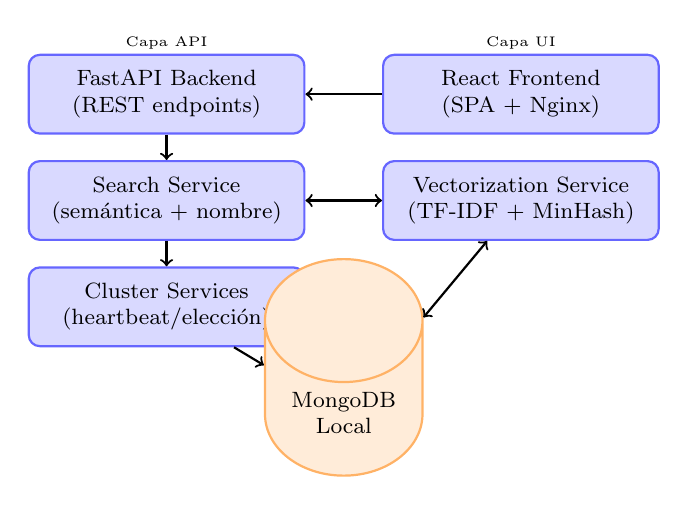
\begin{tikzpicture}[scale=0.9, node distance=1.5cm]
  \tikzstyle{component}=[rectangle, draw=blue!60, fill=blue!15, thick, minimum width=3.5cm, minimum height=1cm, rounded corners, font=\footnotesize, align=center]
  \tikzstyle{storage}=[cylinder, draw=orange!60, fill=orange!15, thick, minimum width=2cm, minimum height=1.2cm, shape border rotate=90, font=\footnotesize, align=center]
  
  % Componentes principales
  \node[component] (api) at (0,4) {FastAPI Backend\\(REST endpoints)};
  \node[component] (search) at (0,2.5) {Search Service\\(semántica + nombre)};
  \node[component] (cluster) at (0,1) {Cluster Services\\(heartbeat/elección)};
  \node[component] (frontend) at (5,4) {React Frontend\\(SPA + Nginx)};
  \node[component] (embed) at (5,2.5) {Vectorization Service\\(TF-IDF + MinHash)};
  
  % Almacenamiento
  \node[storage] (mongo) at (2.5,-0.5) {MongoDB\\Local};
  
  % Conexiones
  \draw[->, thick] (api) -- (search);
  \draw[->, thick] (search) -- (cluster);
  \draw[->, thick] (cluster) -- (mongo);
  \draw[<->, thick] (search) -- (embed);
  \draw[->, thick] (frontend) -- (api);
  \draw[<->, thick] (embed) -- (mongo);
  
  % Etiquetas
  \node[above, font=\tiny] at (0,4.5) {Capa API};
  \node[above, font=\tiny] at (5,4.5) {Capa UI};
\end{tikzpicture}
\caption{Arquitectura de un Slave: integra backend, frontend, búsqueda semántica y servicios de clúster}
\label{fig:peer-architecture}
\end{figure}

\subsection{Patrones de diseño aplicados}

Los siguientes patrones de diseño se aplican siguiendo las mejores prácticas de sistemas distribuidos (Tanenbaum \& Van Steen, 2017):

\begin{description}
  \item[Event-Driven Architecture] \textemdash\ Cada componente reacciona a eventos (llegada de mensajes, timeouts, cambios de estado). FastAPI utiliza un event loop \texttt{asyncio} para multiplexar I/O.
  \item[Message Passing] \textemdash\ Comunicación entre componentes mediante colas de mensajes asíncronas (\texttt{asyncio.Queue}).
  \item[Reactor Pattern] \textemdash\ Event loop que multiplexea I/O de múltiples sockets usando \texttt{uvloop} o \texttt{selectors}.
  \item[Strategy Pattern] \textemdash\ Algoritmos de routing y replicación intercambiables (VIP vs DNSRR, afinidad vs round-robin).
  \item[Observer Pattern] \textemdash\ Notificación de cambios de estado de red a componentes interesados mediante callbacks async.
  \item[Circuit Breaker] \textemdash\ Protección contra cascadas de fallos en llamadas entre servicios.
\end{description}

\subsection{Modelo de concurrencia}

\begin{figure}[H]
\centering
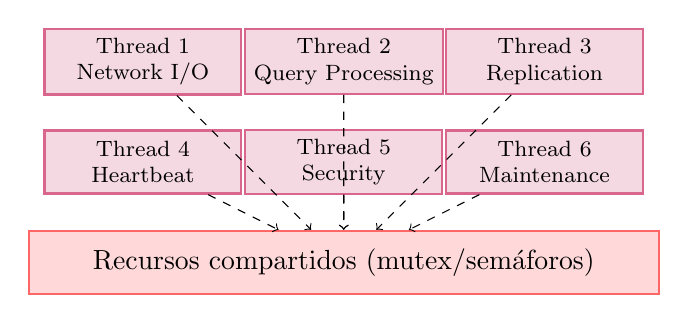
\begin{tikzpicture}[scale=0.85]
  \tikzstyle{thread}=[rectangle, draw=purple!60, fill=purple!15, thick, minimum width=2.5cm, minimum height=0.8cm, font=\footnotesize, align=center]
  
  \node[thread] (t1) at (0,3) {Thread 1\\Network I/O};
  \node[thread] (t2) at (3,3) {Thread 2\\Query Processing};
  \node[thread] (t3) at (6,3) {Thread 3\\Replication};
  \node[thread] (t4) at (0,1.5) {Thread 4\\Heartbeat};
  \node[thread] (t5) at (3,1.5) {Thread 5\\Security};
  \node[thread] (t6) at (6,1.5) {Thread 6\\Maintenance};
  
  % Recursos compartidos
  \node[rectangle, draw=red!60, fill=red!15, thick, minimum width=8cm, minimum height=0.8cm] (shared) at (3,0) {Recursos compartidos (mutex/semáforos)};
  
  \draw[->, dashed] (t1) -- (shared);
  \draw[->, dashed] (t2) -- (shared);
  \draw[->, dashed] (t3) -- (shared);
  \draw[->, dashed] (t4) -- (shared);
  \draw[->, dashed] (t5) -- (shared);
  \draw[->, dashed] (t6) -- (shared);
\end{tikzpicture}
\caption{Modelo de threads para manejo concurrente de operaciones}
\label{fig:concurrency}
\end{figure}

\section{Comunicación entre nodos}

\subsection{Modelo de comunicación por capas}

El sistema implementa una \textbf{arquitectura en capas} para la comunicación siguiendo el modelo OSI adaptado a sistemas distribuidos (Tanenbaum \& Van Steen, 2017). La \textbf{capa de aplicación} define un protocolo de mensajería de alto nivel con mensajes como \texttt{REGISTER}, \texttt{HEARTBEAT}, \texttt{ELECTION}, \texttt{REPLICATE} y \texttt{QUERY}. Esta capa contiene la lógica de coordinación Master-Slave, ubicación semántica de recursos y gestión de estado del clúster.

La \textbf{capa de transporte} utiliza:
\begin{itemize}
  \item \textbf{HTTP/REST (TCP)}: Para operaciones de API síncronas (registro de documentos, consultas)
  \item \textbf{gRPC (HTTP/2)}: Para comunicación inter-nodo de alta eficiencia con Protocol Buffers
  \item \textbf{UDP}: Para heartbeats con baja latencia y tolerancia a pérdidas ocasionales
\end{itemize}

La \textbf{capa de red} utiliza las redes overlay de Docker Swarm con VXLAN. El \textbf{DNS interno de Docker} (\texttt{127.0.0.11}) resuelve nombres de servicio automáticamente:
\begin{itemize}
  \item \texttt{master} $\rightarrow$ VIP del servicio Master
  \item \texttt{slave} $\rightarrow$ VIP balanceada entre réplicas de Slaves
  \item \texttt{tasks.slave} $\rightarrow$ Todas las IPs individuales (modo DNSRR)
\end{itemize}

\subsection{Tipos de comunicación}

\subsubsection{Comunicación Master-Slave (RPC y REST)}
Los Slaves se comunican con el Master mediante \textbf{REST API} (JSON sobre HTTP) para operaciones estándar y \textbf{gRPC} para operaciones de alto rendimiento:
\begin{itemize}
  \item \texttt{POST /register}: Registrar nuevos documentos (el Master actualiza su índice TF-IDF)
  \item \texttt{gRPC ReplicateStream}: Streaming bidireccional para sincronización de réplicas
  \item \texttt{GET /health}: Health checks para el balanceador de Swarm
\end{itemize}

El Master utiliza el DNS de Docker Swarm para descubrir Slaves: \texttt{dns.resolver.query('tasks.slave', 'A')} retorna todas las IPs de réplicas activas.

\subsubsection{Comunicación Slave-Slave}
Los Slaves se comunican entre sí para: heartbeats UDP (detección de fallos), mensajes de elección (algoritmo Bully cuando el Master falla), y transferencia directa de réplicas mediante gRPC streams. Esta comunicación no pasa por el Master, garantizando continuidad ante fallos del coordinador.

\subsubsection{Comunicación Cliente-Sistema}
Los usuarios acceden al sistema a través del \textbf{ingress network} de Docker Swarm. El routing mesh recibe peticiones en cualquier nodo del Swarm y las enruta automáticamente a un Slave disponible mediante IPVS. Externamente se puede configurar un load balancer (HAProxy, Traefik) que resuelve \texttt{distrisearch.local}.

\subsection{Protocolo de mensajería}
Se definen los siguientes tipos de mensajes:

\begin{table}[H]
\centering
\begin{tabularx}{\textwidth}{|l|X|}
\hline
\textbf{Mensaje} & \textbf{Descripción} \\ \hline
\texttt{REGISTER(doc\_id, embedding)} & Slave notifica al Master sobre nuevo documento con su embedding semántico \\ \hline
\texttt{HEARTBEAT(node\_id, status)} & Slave envía estado de salud al Master y otros Slaves (UDP) \\ \hline
\texttt{ELECTION(node\_id)} & Mensaje del algoritmo Bully: inicio de elección de nuevo Master \\ \hline
\texttt{OK(node\_id)} & Respuesta en elección: nodo con ID mayor responde que tomará el liderazgo \\ \hline
\texttt{COORDINATOR(node\_id)} & Anuncio del nuevo Master elegido a todos los Slaves \\ \hline
\texttt{REPLICATE(doc\_id, data, target)} & Instrucción de replicar documento hacia Slave objetivo \\ \hline
\texttt{QUERY(embedding, top\_k)} & Consulta semántica: Master enruta a Slaves con contenido similar \\ \hline
\end{tabularx}
\caption{Tipos de mensajes del protocolo Master-Slave}
\label{tab:messages}
\end{table}

\subsection{Algoritmo de elección de líder: Bully}
Cuando un Slave detecta que el Master no responde (timeout en heartbeats):

\begin{algorithm}[H]
\caption{Algoritmo Bully para elección de Master}
\begin{algorithmic}[1]
\State \textbf{Input:} nodo actual $P_i$, conjunto de nodos $\{P_1, ..., P_n\}$ ordenados por ID
\State $P_i$ envía mensaje ELECTION a todos $P_j$ donde $j > i$
\If{ningún $P_j$ responde con OK en timeout}
    \State $P_i$ se convierte en Master
    \State $P_i$ envía COORDINATOR a todos los nodos
\Else
    \State $P_i$ espera mensaje COORDINATOR del nodo con mayor ID
\EndIf
\end{algorithmic}
\end{algorithm}

\textbf{Ejemplo}: Si el Master (ID=100) falla y los Slaves tienen IDs 50, 60, 70:
\begin{enumerate}
  \item Slave-50 detecta fallo, envía ELECTION a 60, 70
  \item Slave-60 y 70 responden OK (tienen ID mayor)
  \item Slave-60 envía ELECTION a 70
  \item Slave-70 responde OK
  \item Slave-70 no tiene nadie con ID mayor, se convierte en Master
  \item Slave-70 envía COORDINATOR a todos: nuevo Master elegido
\end{enumerate}

\section{Coordinación y sincronización}

\subsection{Modelo de coordinación}

La coordinación en sistemas distribuidos aborda dos problemas fundamentales: el ordenamiento de eventos y la toma de decisiones colectivas (Tanenbaum \& Van Steen, 2017). El sistema DistriSearch implementa mecanismos específicos para cada uno.

\subsubsection{Desacoplamiento temporal y referencial}

El sistema implementa diferentes niveles de acoplamiento según el tipo de operación:

\begin{table}[H]
\centering
\begin{tabularx}{\textwidth}{|l|X|X|}
\hline
\textbf{Operación} & \textbf{Acoplamiento temporal} & \textbf{Acoplamiento referencial} \\ \hline
Consulta directa & Acoplado (síncrono) & Acoplado (peer específico) \\ \hline
Replicación & Desacoplado (asíncrono) & Acoplado (réplicas específicas) \\ \hline
Búsqueda flooding & Desacoplado & Parcialmente desacoplado \\ \hline
Heartbeat & Desacoplado & Acoplado (vecinos) \\ \hline
\end{tabularx}
\caption{Niveles de acoplamiento por tipo de operación}
\label{tab:coupling}
\end{table}

El sistema implementa dos modos principales de comunicación con diferentes características de acoplamiento. La \textbf{comunicación directa} es temporalmente acoplada, lo que significa que ambos nodos (emisor y receptor) deben estar activos simultáneamente para completar la interacción. También es referencialmente acoplada porque el emisor conoce explícitamente la identidad del receptor. Este modo se utiliza para consultas síncronas donde se espera una respuesta inmediata y para transferencias de datos que requieren confirmación.

Por otro lado, la \textbf{comunicación basada en eventos} es temporalmente desacoplada, permitiendo que publicación y suscripción ocurran en momentos diferentes sin requerir sincronía estricta. También es referencialmente desacoplada ya que los publicadores no necesitan conocer la identidad de los suscriptores. Este patrón se emplea para notificaciones de cambios de estado, detección de fallos y propagación de eventos que múltiples nodos pueden consumir.

\subsection{Sincronización de acciones}

\subsubsection{Protocolo de sincronización para operaciones distribuidas}

\textbf{Relojes Lógicos de Lamport (1978):} El sistema utiliza relojes lógicos para establecer un ordenamiento parcial de eventos distribuidos, fundamental para la consistencia de operaciones (Tanenbaum \& Van Steen, 2017). Cada nodo mantiene un contador $L_i$ que se incrementa en cada evento local según las siguientes reglas:

\begin{enumerate}
  \item \textbf{Evento local}: $L_i := L_i + 1$
  \item \textbf{Envío de mensaje}: Incrementar $L_i$, adjuntar timestamp $T = L_i$ al mensaje
  \item \textbf{Recepción de mensaje} con timestamp $T$: $L_i := \max(L_i, T) + 1$
\end{enumerate}

Este mecanismo garantiza la propiedad de \textbf{causalidad}: si un evento $a$ causalmente precede a un evento $b$ (notado $a \rightarrow b$), entonces $L(a) < L(b)$. Para resolver empates cuando dos eventos tienen el mismo timestamp, se utiliza el identificador del nodo como criterio de desempate: $(T_1, node_1) < (T_2, node_2)$ si $T_1 < T_2$, o si $T_1 = T_2$ y $node_1 < node_2$.

\textbf{Aplicación en DistriSearch:} Los timestamps de Lamport se utilizan para:
\begin{itemize}
  \item Ordenar operaciones de replicación concurrentes
  \item Detectar mensajes de elección obsoletos
  \item Resolver conflictos en actualizaciones del índice semántico
\end{itemize}

\subsection{Toma de decisiones distribuidas}

\subsubsection{Algoritmo Bully para elección de líder}

El algoritmo Bully (Garcia-Molina, 1982) se utiliza para elegir un nuevo Master cuando el actual falla. Es un algoritmo de elección que garantiza que el nodo con mayor ID (prioridad) se convierte en líder.

\subsubsection{Consenso Raft-Lite para operaciones críticas}

Para operaciones que requieren acuerdo entre múltiples nodos, el sistema implementa una versión simplificada del algoritmo \textbf{Raft} (Ongaro \& Ousterhout, 2014), adaptada para el contexto Master-Slave:

\begin{enumerate}
  \item \textbf{Términos (Terms)}: Cada período de liderazgo tiene un número de término monotonamente creciente
  \item \textbf{Heartbeats del líder}: El Master envía heartbeats periódicos a todos los Slaves
  \item \textbf{Timeout de elección}: Si un Slave no recibe heartbeat en $T_{election}$, inicia elección
  \item \textbf{Votación}: Cada Slave vota por el primer candidato que solicita voto en un término
  \item \textbf{Mayoría}: Candidato con $> N/2$ votos se convierte en líder
\end{enumerate}

\textbf{Consenso para cambios de configuración:}
\begin{itemize}
  \item Cambios críticos (ej: modificar factor de replicación) requieren consenso
  \item Se usa votación de mayoría simple: solo se aplica cambio si $> 50\%$ de nodos activos aprueban
  \item Los cambios se registran en un log replicado para recuperación ante fallos
\end{itemize}

\section{Localización y nombrado de datos / recursos}

El sistema de nombrado y localización combina dos mecanismos complementarios (Tanenbaum \& Van Steen, 2017):

\subsection{Nombrado basado en DNS de Docker Swarm}

Docker Swarm proporciona un sistema de nombrado jerárquico automático:
\begin{itemize}
  \item \textbf{Nombres de servicio}: \texttt{master}, \texttt{slave}, \texttt{mongo} resueltos por DNS interno
  \item \textbf{Nombres de tareas}: \texttt{slave.1}, \texttt{slave.2}, etc. para acceso a réplicas específicas
  \item \textbf{DNS queries}: \texttt{tasks.slave} retorna todas las IPs (DNSRR)
\end{itemize}

\subsection{Localización semántica con TF-IDF + MinHash}

Cada documento tiene un identificador único (UUID) y un \textbf{vector TF-IDF} que representa su contenido. A diferencia de embeddings de redes neuronales pre-entrenadas, TF-IDF ofrece:
\begin{itemize}
  \item \textbf{Interpretabilidad}: Pesos directamente relacionados con términos del documento
  \item \textbf{Eficiencia}: Cálculo local sin dependencia de modelos externos
  \item \textbf{Extensibilidad}: Fácil actualización del vocabulario global
\end{itemize}

Para detección rápida de similitud, se utiliza \textbf{MinHash} (Broder, 1997) que genera firmas compactas de 128 hashes para cada documento, permitiendo estimar similitud Jaccard en $O(1)$.

El Master mantiene un \textbf{índice de ubicación semántica} que mapea cada Slave a un perfil TF-IDF agregado de sus documentos. Cuando llega una consulta, el Master calcula su vector TF-IDF y determina qué Slaves tienen contenido semánticamente similar usando similitud coseno.

\subsection{Particionamiento con VP-Tree y Centroides}

El sistema utiliza un \textbf{VP-Tree} (Vantage-Point Tree) para particionar el espacio semántico de documentos (Yianilos, 1993). A diferencia de estructuras como KD-Trees que trabajan bien en espacios de baja dimensión, VP-Tree escala eficientemente en espacios métricos de alta dimensión típicos de representaciones TF-IDF.

\subsubsection{Estructura del VP-Tree}

El VP-Tree divide recursivamente el espacio de documentos:
\begin{enumerate}
  \item Se selecciona un \textbf{vantage point} (punto de referencia) como pivote
  \item Se calcula la \textbf{distancia mediana} $\mu$ de todos los documentos al pivote
  \item Los documentos con $d(x, vp) \leq \mu$ van al subárbol izquierdo
  \item Los documentos con $d(x, vp) > \mu$ van al subárbol derecho
  \item Se repite recursivamente hasta que cada hoja contiene $\leq$ threshold documentos
\end{enumerate}

\begin{algorithm}[H]
\caption{Construcción de VP-Tree para particionamiento}
\begin{algorithmic}[1]
\Function{BuildVPTree}{$documents$}
  \If{$|documents| \leq threshold$}
    \State \Return \textbf{Leaf}($documents$, centroid=\Call{ComputeCentroid}{$documents$})
  \EndIf
  \State $vp \gets$ \Call{SelectVantagePoint}{$documents$}  \Comment{Maximiza varianza de distancias}
  \State $distances \gets [d(doc, vp)$ for $doc$ in $documents]$
  \State $\mu \gets$ median($distances$)
  \State $left \gets \{doc : d(doc, vp) \leq \mu\}$
  \State $right \gets \{doc : d(doc, vp) > \mu\}$
  \State \Return \textbf{Node}($vp$, $\mu$, \Call{BuildVPTree}{$left$}, \Call{BuildVPTree}{$right$})
\EndFunction
\end{algorithmic}
\end{algorithm}

\subsubsection{Centroides de partición}

Cada partición (hoja del VP-Tree) tiene un \textbf{centroide} que representa el perfil semántico agregado de sus documentos. El centroide se calcula como la media de los vectores TF-IDF normalizados:

$$\text{centroid}_p = \frac{1}{|D_p|} \sum_{d \in D_p} \frac{\mathbf{v}_d}{\|\mathbf{v}_d\|_2}$$

donde $D_p$ es el conjunto de documentos en la partición $p$ y $\mathbf{v}_d$ es el vector TF-IDF del documento $d$.

\textbf{Recomputación de centroides}: Cuando la distribución de documentos en una partición cambia significativamente (drift semántico), se ejecuta un algoritmo de \textbf{k-medoids} para recomputar centroides óptimos:

\begin{algorithm}[H]
\caption{Recomputación de centroides con k-medoids}
\begin{algorithmic}[1]
\Function{RecomputeCentroids}{$partitions$, $k$}
  \For{$partition$ in $partitions$}
    \If{$partition.drift\_score > threshold$}
      \State $medoids \gets$ \Call{KMedoids}{$partition.documents$, $k=1$}
      \State $partition.centroid \gets medoids[0]$
      \State $partition.drift\_score \gets 0$
    \EndIf
  \EndFor
\EndFunction
\end{algorithmic}
\end{algorithm}

\subsubsection{LSH para agrupamiento de documentos similares}

\textbf{Locality-Sensitive Hashing (LSH)} se utiliza para pre-agrupar documentos similares antes de su asignación a particiones (Indyk \& Motwani, 1998). LSH garantiza que documentos con alta similitud Jaccard tengan alta probabilidad de colisionar en el mismo bucket:

$$P[\text{hash}(a) = \text{hash}(b)] = J(a, b)$$

donde $J(a,b)$ es la similitud Jaccard entre documentos $a$ y $b$.

El sistema implementa LSH con \textbf{bandas} (banding technique):
\begin{itemize}
  \item Las 128 firmas MinHash se dividen en $b=16$ bandas de $r=8$ hashes cada una
  \item Dos documentos son \textbf{candidatos similares} si coinciden en al menos una banda completa
  \item Probabilidad de ser candidatos: $P = 1 - (1 - s^r)^b$ donde $s$ es la similitud real
  \item Con $b=16, r=8$: documentos con $s \geq 0.5$ tienen $>96\%$ de probabilidad de ser candidatos
\end{itemize}

\begin{figure}[H]
\centering
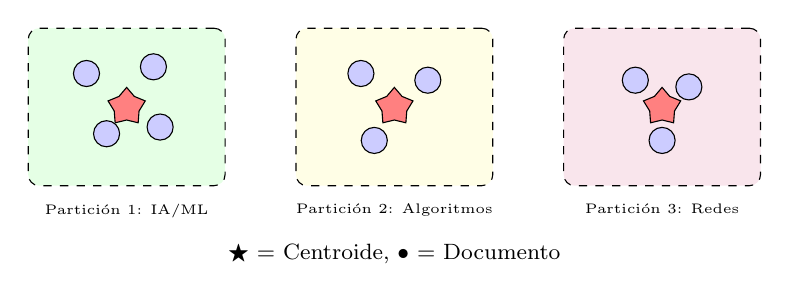
\begin{tikzpicture}[scale=0.85]
  \tikzstyle{doc}=[circle, draw, fill=blue!20, minimum size=0.3cm]
  \tikzstyle{centroid}=[star, star points=5, draw, fill=red!50, minimum size=0.4cm]
  \tikzstyle{partition}=[rectangle, draw, dashed, rounded corners]
  
  % Partición 1 (IA/ML)
  \node[partition, minimum width=2.5cm, minimum height=2cm, fill=green!10] (p1) at (0,0) {};
  \node[centroid] (c1) at (0,0) {};
  \node[doc] at (-0.6,0.5) {};
  \node[doc] at (0.4,0.6) {};
  \node[doc] at (-0.3,-0.4) {};
  \node[doc] at (0.5,-0.3) {};
  \node[font=\tiny, below] at (0,-1.3) {Partición 1: IA/ML};
  
  % Partición 2 (Algoritmos)
  \node[partition, minimum width=2.5cm, minimum height=2cm, fill=yellow!10] (p2) at (4,0) {};
  \node[centroid] (c2) at (4,0) {};
  \node[doc] at (3.5,0.5) {};
  \node[doc] at (4.5,0.4) {};
  \node[doc] at (3.7,-0.5) {};
  \node[font=\tiny, below] at (4,-1.3) {Partición 2: Algoritmos};
  
  % Partición 3 (Redes)
  \node[partition, minimum width=2.5cm, minimum height=2cm, fill=purple!10] (p3) at (8,0) {};
  \node[centroid] (c3) at (8,0) {};
  \node[doc] at (7.6,0.4) {};
  \node[doc] at (8.4,0.3) {};
  \node[doc] at (8,-0.5) {};
  \node[font=\tiny, below] at (8,-1.3) {Partición 3: Redes};
  
  % Leyenda
  \node[font=\footnotesize] at (4,-2.2) {$\bigstar$ = Centroide, $\bullet$ = Documento};
\end{tikzpicture}
\caption{Particiones VP-Tree con centroides representando regiones semánticas}
\label{fig:vptree-partitions}
\end{figure}

\subsection{Rebalanceo activo de particiones}

Cuando un nodo se une o abandona el clúster, el sistema ejecuta un \textbf{rebalanceo activo} para redistribuir documentos. El algoritmo utiliza la técnica \textbf{"Power of Two Choices"} con afinidad semántica:

\begin{algorithm}[H]
\caption{Rebalanceo activo con Power of Two Choices}
\begin{algorithmic}[1]
\Function{Rebalance}{$cluster$, $event$}
  \If{$event.type = $ NODE\_JOIN}
    \State $overloaded \gets$ \Call{GetOverloadedNodes}{$cluster$}
    \For{$node$ in $overloaded$}
      \State $docs\_to\_migrate \gets$ \Call{SelectMigrationCandidates}{$node$}
      \For{$doc$ in $docs\_to\_migrate$}
        \State $choice1, choice2 \gets$ \Call{RandomSample}{$cluster.nodes$, 2}
        \State $best \gets$ node con menor carga Y mayor afinidad semántica con $doc$
        \State \Call{Migrate}{$doc$, $node$, $best$}
      \EndFor
    \EndFor
  \ElsIf{$event.type = $ NODE\_LEAVE}
    \State $orphan\_docs \gets event.node.documents$
    \For{$doc$ in $orphan\_docs$}
      \State $target \gets$ \Call{FindBestNode}{$doc$, $cluster$}  \Comment{Por afinidad}
      \State \Call{RestoreFromReplica}{$doc$, $target$}
    \EndFor
  \EndIf
\EndFunction
\end{algorithmic}
\end{algorithm}

\textbf{Métricas para selección de nodo destino}:
\begin{itemize}
  \item \textbf{Score de afinidad}: $\text{affinity}(doc, node) = \cos(\mathbf{v}_{doc}, \text{centroid}_{node})$
  \item \textbf{Score de carga}: $\text{load}(node) = \frac{\text{docs\_count}}{\text{capacity}}$
  \item \textbf{Score combinado}: $\alpha \cdot \text{affinity} + (1-\alpha) \cdot (1 - \text{load})$ con $\alpha = 0.6$
\end{itemize}

\subsection{Estrategias de localización de datos}

\subsubsection{Estrategia 1: Búsqueda semántica centralizada con TF-IDF}
\begin{algorithm}[H]
\caption{Búsqueda semántica en Master usando TF-IDF + MinHash}
\begin{algorithmic}[1]
\State \textbf{Input:} $query$ (texto de consulta), $top\_k$ (número de resultados)
\State \textbf{Output:} lista de documentos relevantes
\State $q\_tfidf \gets$ calcular\_tfidf($query$, $vocabulario\_global$)
\State $q\_minhash \gets$ calcular\_minhash($query$)
\State \Comment{Fase 1: Filtrado rápido con MinHash}
\State $candidatos \gets$ filtrar\_por\_minhash($q\_minhash$, $umbral\_jaccard=0.3$)
\State \Comment{Fase 2: Ranking preciso con TF-IDF}
\State $slaves \gets$ ordenar\_slaves\_por\_similitud\_coseno($q\_tfidf$, $candidatos$)
\State $results \gets []$
\For{$slave$ en $slaves[:3]$}  \Comment{Top 3 Slaves más relevantes}
    \State $local\_results \gets$ enviar\_query\_grpc($slave$, $query$)
    \State $results \gets results \cup local\_results$
\EndFor
\State \Return ordenar\_por\_relevancia($results$)[:$top\_k$]
\end{algorithmic}
\end{algorithm}

\subsubsection{Estrategia 2: Asignación por afinidad semántica}
Asignar cada documento al Slave cuyo perfil TF-IDF es más similar:
$$\text{slave\_destino} = \arg\max_{s \in \text{slaves}} \cos(tfidf_{doc}, profile_s)$$
donde $\cos$ es la similitud coseno entre vectores TF-IDF.

\textbf{Ejemplo}: Un documento sobre "algoritmos de ordenamiento" tiene un vector TF-IDF que el Master compara con los perfiles de cada Slave. Si Slave-2 ya contiene documentos sobre "estructuras de datos" y "complejidad algorítmica", su perfil TF-IDF tendrá términos similares, por lo que el nuevo documento se almacena allí.

\begin{figure}[H]
\centering
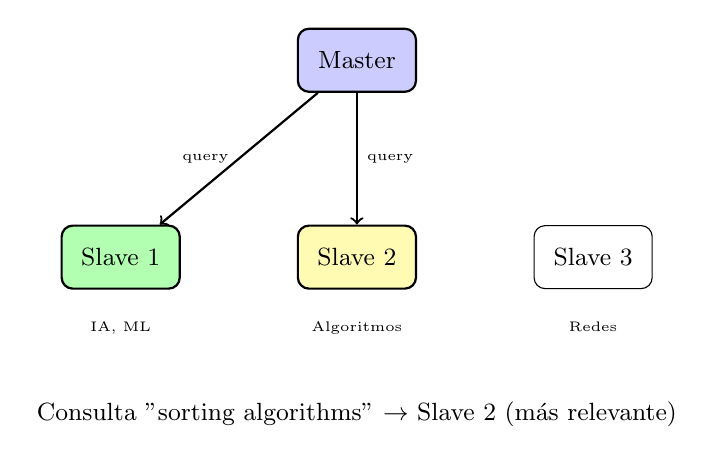
\begin{tikzpicture}[scale=1.0]
  \tikzstyle{node}=[rectangle, draw, minimum width=1.5cm, minimum height=0.8cm, font=\small, rounded corners]
  \tikzstyle{master}=[fill=blue!20, thick]
  \tikzstyle{primary}=[fill=green!30, thick]
  \tikzstyle{replica}=[fill=yellow!30, thick]
  
  % Master
  \node[node, master] (m) at (3,4) {Master};
  
  % Slaves
  \node[node, primary] (s1) at (0,1.5) {Slave 1};
  \node[node, replica] (s2) at (3,1.5) {Slave 2};
  \node[node] (s3) at (6,1.5) {Slave 3};
  
  % Perfiles semánticos
  \node[font=\tiny, below] at (0,0.8) {IA, ML};
  \node[font=\tiny, below] at (3,0.8) {Algoritmos};
  \node[font=\tiny, below] at (6,0.8) {Redes};
  
  % Conexiones
  \draw[->, thick] (m) -- node[left, font=\tiny] {query} (s1);
  \draw[->, thick] (m) -- node[right, font=\tiny] {query} (s2);
  
  % Leyenda
  \node[font=\small] at (3,-0.5) {Consulta "sorting algorithms" $\rightarrow$ Slave 2 (más relevante)};
\end{tikzpicture}
\caption{Ubicación semántica: Master enruta consultas a Slaves con contenido similar}
\label{fig:data-location}
\end{figure}

\section{Distribución, replicación y consistencia de datos}

La replicación es fundamental para garantizar disponibilidad y tolerancia a fallos en sistemas distribuidos (Tanenbaum \& Van Steen, 2017). El sistema implementa replicación donde cada documento puede tener $k$ réplicas en diferentes Slaves (por defecto $k = 2$). El coordinador de replicación en el Master selecciona Slaves con \textbf{afinidad semántica basada en TF-IDF}: documentos similares se replican en Slaves que ya contienen contenido relacionado, mejorando la localidad de las consultas.

Respecto a la consistencia, los documentos son inmutables una vez subidos, simplificando el modelo al eliminar la necesidad de sincronizar actualizaciones (modelo WORM: Write Once, Read Many).

\subsection{Estrategia de replicación por afinidad semántica}
Para un factor de replicación $k=2$, al almacenar un documento en el Slave primario $S_p$, el Master selecciona $k-1 = 1$ Slaves adicionales para réplicas. Los criterios de selección son:
\begin{itemize}
  \item \textbf{Afinidad semántica}: Preferir Slaves cuyo perfil TF-IDF sea similar al vector del documento
  \item \textbf{Carga actual}: Balancear distribución de almacenamiento entre Slaves (métrica: GB usados)
  \item \textbf{Disponibilidad}: Priorizar Slaves con historial de uptime alto (ventana de 24h)
\end{itemize}

\begin{figure}[H]
\centering
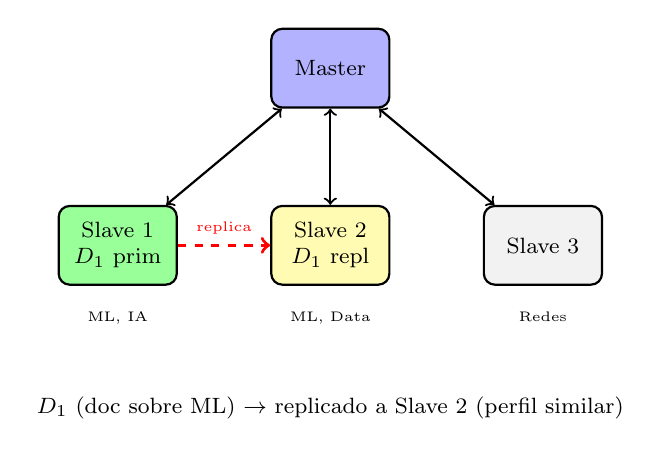
\begin{tikzpicture}[scale=0.9]
  \tikzstyle{node}=[rectangle, draw, thick, minimum width=1.5cm, minimum height=1cm, font=\footnotesize, align=center, rounded corners]
  \tikzstyle{master}=[fill=blue!30]
  \tikzstyle{primary}=[fill=green!40]
  \tikzstyle{replica}=[fill=yellow!30]
  \tikzstyle{normal}=[fill=gray!10]
  
  % Master
  \node[node, master] (m) at (3,4) {Master};
  
  % Slaves
  \node[node, primary] (s1) at (0,1.5) {Slave 1\\$D_1$ prim};
  \node[node, replica] (s2) at (3,1.5) {Slave 2\\$D_1$ repl};
  \node[node, normal] (s3) at (6,1.5) {Slave 3};
  
  % Perfiles
  \node[font=\tiny, below] at (0,0.7) {ML, IA};
  \node[font=\tiny, below] at (3,0.7) {ML, Data};
  \node[font=\tiny, below] at (6,0.7) {Redes};
  
  % Conexiones
  \draw[<->, thick] (m) -- (s1);
  \draw[<->, thick] (m) -- (s2);
  \draw[<->, thick] (m) -- (s3);
  
  % Flecha de replicación
  \draw[->, very thick, red, dashed] (s1) -- node[midway, above] {\tiny replica} (s2);
  
  % Leyenda
  \node[font=\footnotesize, below] at (3,-0.5) {$D_1$ (doc sobre ML) $\rightarrow$ replicado a Slave 2 (perfil similar)};
\end{tikzpicture}
\caption{Replicación por afinidad semántica: documento ML replicado a Slave con perfil similar}
\label{fig:replication}
\end{figure}

\subsection{Modelo de consistencia}

El sistema adopta un modelo de \textbf{consistencia eventual} (Tanenbaum \& Van Steen, 2017), priorizando disponibilidad y tolerancia a particiones (teorema CAP):

\begin{itemize}
  \item \textbf{Escrituras}: Documentos nuevos se escriben primero en el Slave que recibe la subida (\textit{primary}), luego se replican asíncronamente a réplicas secundarias
  \item \textbf{Lecturas}: Cualquier Slave con una réplica puede responder consultas (\textit{read-any})
  \item \textbf{Convergencia}: Garantizada por la naturaleza inmutable de los documentos
  \item \textbf{Ventana de inconsistencia}: Típicamente $< 5s$ bajo condiciones normales de red
\end{itemize}

\subsubsection{Garantías de durabilidad}
\begin{itemize}
  \item \textbf{At-least-once delivery}: Replicación con ACKs y reintentos automáticos
  \item \textbf{Quorum writes}: Opcionalmente, escritura confirmada solo si $\geq k/2 + 1$ réplicas confirman
  \item \textbf{Anti-entropy}: Reconciliación periódica entre réplicas usando MinHash para detección de divergencias
\end{itemize}

\section{Tolerancia a fallos, robustez y dinámicas de red}

La tolerancia a fallos parciales es una característica esencial de los sistemas distribuidos (Tanenbaum \& Van Steen, 2017). El sistema DistriSearch proporciona soporte integral para: Slaves que se desconectan temporalmente, fallo del Master (recuperado mediante elección Bully), particiones de red, y reincorporación de nodos nuevos o recuperados.

\subsection{Modelo de fallos}
El sistema asume un modelo de \textbf{fail-stop} donde los nodos fallan deteniendo su ejecución completamente (no hay comportamiento bizantino). Los fallos se clasifican en:
\begin{itemize}
  \item \textbf{Crash failures}: El nodo deja de responder y no se recupera
  \item \textbf{Omission failures}: Pérdida de mensajes (mitigado con reintentos)
  \item \textbf{Timing failures}: Respuestas fuera de timeout (detectado por heartbeats)
\end{itemize}

La arquitectura Master-Slave con elección de líder garantiza continuidad: si el Master falla, los Slaves detectan la ausencia de heartbeats y ejecutan el algoritmo Bully para elegir un nuevo coordinador.

\subsection{Dinámicas de red en Docker Swarm}
Cuando un Slave nuevo se une a la red o un Slave existente falla, Docker Swarm gestiona automáticamente parte del proceso:
\begin{itemize}
  \item \textbf{Nuevo Slave}: Swarm lo añade a la red overlay, DNS interno actualiza registros automáticamente
  \item \textbf{Registro con Master}: El nuevo Slave envía su perfil TF-IDF inicial vía REST API
  \item \textbf{Fallo de Slave}: El Master detecta ausencia de heartbeats (timeout 15s) y marca el nodo como no disponible
  \item \textbf{Health checks de Swarm}: Docker también detecta fallos y puede reiniciar contenedores automáticamente
  \item \textbf{Fallo de Master}: Slaves detectan timeout, inician elección Bully, nuevo Master asume coordinación
  \item \textbf{Re-replicación}: Si un Slave con réplicas falla permanentemente, el Master coordina crear nuevas réplicas
\end{itemize}

\subsection{Detección de fallos mediante Heartbeat}
\begin{algorithm}[H]
\caption{Protocolo Heartbeat para detección de fallos}
\begin{algorithmic}[1]
\State \textbf{Constantes:} $T_{heartbeat} = 5s$, $T_{timeout} = 15s$
\While{nodo está activo}
    \For{cada vecino $v$ en lista de vecinos}
        \State Enviar \texttt{PING} a $v$
        \If{no se recibe \texttt{PONG} en $T_{timeout}$}
            \State Marcar $v$ como fallido
            \State Notificar a otros vecinos sobre fallo de $v$
            \State Intentar reconexión o buscar reemplazo
        \EndIf
    \EndFor
    \State Esperar $T_{heartbeat}$
\EndWhile
\end{algorithmic}
\end{algorithm}

\subsection{Protocolo de incorporación de nuevo nodo (JOIN)}
\begin{figure}[H]
\centering
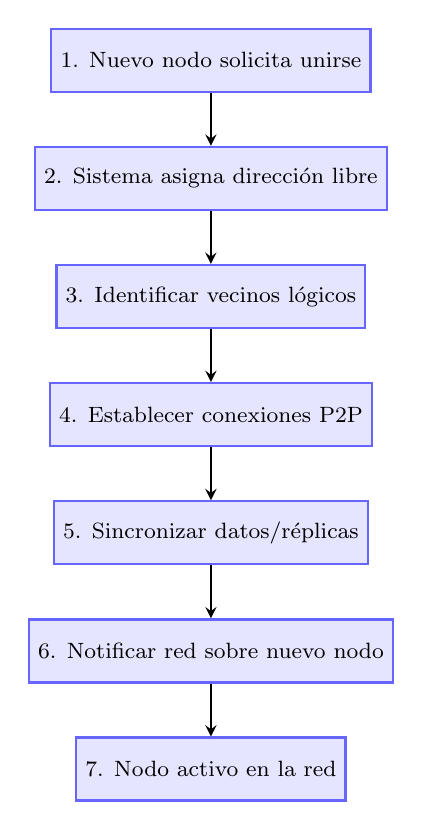
\begin{tikzpicture}[scale=0.8, node distance=1.5cm]
  \tikzstyle{process}=[rectangle, draw=blue!60, fill=blue!10, thick, minimum width=3cm, minimum height=0.8cm, font=\footnotesize, align=center]
  \tikzstyle{arrow}=[->, thick, >=stealth]
  
  \node[process] (s1) {1. Nuevo nodo solicita unirse};
  \node[process, below of=s1] (s2) {2. Sistema asigna dirección libre};
  \node[process, below of=s2] (s3) {3. Identificar vecinos lógicos};
  \node[process, below of=s3] (s4) {4. Establecer conexiones P2P};
  \node[process, below of=s4] (s5) {5. Sincronizar datos/réplicas};
  \node[process, below of=s5] (s6) {6. Notificar red sobre nuevo nodo};
  \node[process, below of=s6] (s7) {7. Nodo activo en la red};
  
  \draw[arrow] (s1) -- (s2);
  \draw[arrow] (s2) -- (s3);
  \draw[arrow] (s3) -- (s4);
  \draw[arrow] (s4) -- (s5);
  \draw[arrow] (s5) -- (s6);
  \draw[arrow] (s6) -- (s7);
\end{tikzpicture}
\caption{Proceso de incorporación de nuevo nodo a la red P2P}
\label{fig:join-protocol}
\end{figure}

\subsection{Manejo de fallo de nodo}
Cuando un nodo $N$ falla:

\begin{enumerate}
  \item \textbf{Detección}: Vecinos detectan fallo por timeout de heartbeat
  \item \textbf{Notificación}: Vecinos notifican al resto de la red
  \item \textbf{Reconexión}: Vecinos de $N$ se conectan entre sí para mantener conectividad
  \item \textbf{Re-replicación}: Datos con réplicas en $N$ se replican en otros nodos
  \item \textbf{Actualización de rutas}: Tablas de routing se actualizan
\end{enumerate}

\begin{figure}[H]
\centering
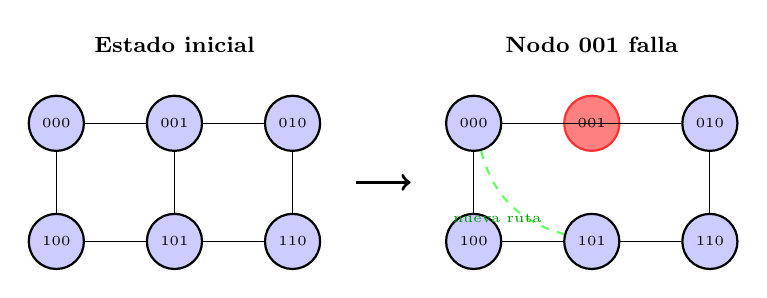
\begin{tikzpicture}[scale=1.0]
  % Estado inicial
  \begin{scope}
    \node[font=\footnotesize\bfseries] at (1.5,2.5) {Estado inicial};
    \tikzstyle{node}=[circle, draw, thick, minimum size=0.7cm, font=\tiny, fill=blue!20]
    \tikzstyle{failed}=[fill=red!50]
    
    \node[node] (a1) at (0,1.5) {000};
    \node[node] (b1) at (1.5,1.5) {001};
    \node[node] (c1) at (3,1.5) {010};
    \node[node] (d1) at (0,0) {100};
    \node[node] (e1) at (1.5,0) {101};
    \node[node] (f1) at (3,0) {110};
    
    \draw[-] (a1) -- (b1);
    \draw[-] (b1) -- (c1);
    \draw[-] (a1) -- (d1);
    \draw[-] (b1) -- (e1);
    \draw[-] (c1) -- (f1);
    \draw[-] (d1) -- (e1);
    \draw[-] (e1) -- (f1);
  \end{scope}
  
  % Flecha de transición
  \draw[->, very thick] (3.8,0.75) -- (4.5,0.75);
  
  % Estado después del fallo
  \begin{scope}[xshift=5.3cm]
    \node[font=\footnotesize\bfseries] at (1.5,2.5) {Nodo 001 falla};
    \tikzstyle{node}=[circle, draw, thick, minimum size=0.7cm, font=\tiny, fill=blue!20]
    \tikzstyle{failed}=[fill=red!50, draw=red!80]
    
    \node[node] (a2) at (0,1.5) {000};
    \node[node, failed] (b2) at (1.5,1.5) {001};
    \node[node] (c2) at (3,1.5) {010};
    \node[node] (d2) at (0,0) {100};
    \node[node] (e2) at (1.5,0) {101};
    \node[node] (f2) at (3,0) {110};
    
    \draw[-] (a2) -- (c2);
    \draw[-] (a2) -- (d2);
    \draw[-] (c2) -- (f2);
    \draw[-] (d2) -- (e2);
    \draw[-] (e2) -- (f2);
    \draw[-, dashed, thick, green!60] (a2) to[bend right=30] (e2);
    
    \node[font=\tiny, green!60!black] at (0.3,0.3) {nueva ruta};
  \end{scope}
\end{tikzpicture}
\caption{Reconfiguración de red tras fallo de nodo 001: rutas alternativas y reconexiones}
\label{fig:fault-tolerance}
\end{figure}

\subsection{Métricas de resiliencia}

Para un clúster con $N$ Slaves, el sistema presenta características de resiliencia cuantificables:
\begin{itemize}
  \item \textbf{Tolerancia a fallos de Slaves}: El sistema permanece operativo mientras al menos un Slave esté activo
  \item \textbf{Tolerancia a fallo de Master}: El algoritmo Bully elige nuevo Master en $O(N)$ mensajes
  \item \textbf{Tiempo de detección de fallo}: Determinado por $T_{timeout} = 15s$ (3 heartbeats perdidos)
  \item \textbf{Tiempo de recuperación}: Elección Bully completa en $< 30s$ típicamente
\end{itemize}

\section{Seguridad, autenticación y autorización}

La seguridad en sistemas distribuidos abarca múltiples dimensiones: confidencialidad, integridad, disponibilidad y autenticación (Tanenbaum \& Van Steen, 2017). El sistema DistriSearch implementa múltiples capas de seguridad aprovechando las capacidades nativas de Docker Swarm.

\subsection{Seguridad en Docker Swarm}

Docker Swarm proporciona mecanismos de seguridad integrados:

\begin{itemize}
  \item \textbf{Cifrado de overlay networks}: Habilitado con \texttt{--opt encrypted}, utiliza IPSec para cifrar todo el tráfico entre nodos del Swarm
  \item \textbf{Mutual TLS (mTLS)}: Comunicación entre nodos del Swarm automáticamente cifrada y autenticada
  \item \textbf{Docker Secrets}: Almacenamiento seguro de credenciales, API keys y certificados, accesibles solo por servicios autorizados
  \item \textbf{Rotación automática de certificados}: Swarm rota certificados TLS cada 90 días (configurable)
\end{itemize}

\begin{verbatim}
# Crear red overlay cifrada
docker network create --driver overlay --opt encrypted \
  distrisearch-secure

# Crear secret para API key
echo "my-api-key" | docker secret create api_key -

# Usar secret en servicio
docker service create --name slave --secret api_key \
  distrisearch/slave:latest
\end{verbatim}

\subsection{Autenticación y autorización a nivel de aplicación}

Cada nodo posee una identidad única basada en criptografía de clave pública (par de claves pública/privada), lo que permite autenticación mutua entre nodos antes de establecer comunicación. El sistema implementa control de acceso mediante:
\begin{itemize}
  \item \textbf{JWT tokens}: Para autenticación de clientes en la API REST
  \item \textbf{API Keys}: Para comunicación inter-servicio con Docker Secrets
  \item \textbf{ACLs}: Listas de control de acceso para operaciones administrativas
\end{itemize}

\subsection{Modelo de seguridad por capas}

\begin{figure}[H]
\centering
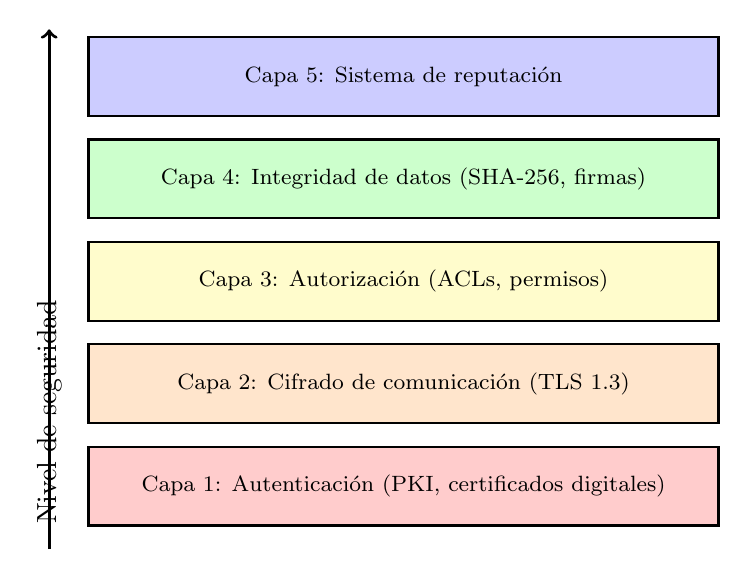
\begin{tikzpicture}[scale=1.0]
  \tikzstyle{layer}=[rectangle, draw, thick, minimum width=8cm, minimum height=1cm, font=\footnotesize]
  
  \node[layer, fill=red!20] (l1) at (0,0) {Capa 1: Autenticación (PKI, certificados digitales)};
  \node[layer, fill=orange!20] (l2) at (0,1.3) {Capa 2: Cifrado de comunicación (TLS 1.3)};
  \node[layer, fill=yellow!20] (l3) at (0,2.6) {Capa 3: Autorización (ACLs, permisos)};
  \node[layer, fill=green!20] (l4) at (0,3.9) {Capa 4: Integridad de datos (SHA-256, firmas)};
  \node[layer, fill=blue!20] (l5) at (0,5.2) {Capa 5: Sistema de reputación};
  
  \draw[->, very thick] (-4.5,-0.8) -- (-4.5,5.8) node[midway, left, rotate=90] {Nivel de seguridad};
\end{tikzpicture}
\caption{Arquitectura de seguridad por capas}
\label{fig:security-layers}
\end{figure}

\subsection{Protocolo de autenticación}

\begin{algorithm}[H]
\caption{Autenticación mutua entre peers}
\begin{algorithmic}[1]
\State \textbf{Nodo A quiere conectarse con Nodo B}
\State A genera nonce $N_A$ aleatorio
\State A $\rightarrow$ B: \texttt{HELLO}($ID_A$, $N_A$, $Cert_A$)
\State B verifica $Cert_A$ con autoridad certificadora
\If{$Cert_A$ es válido}
    \State B genera nonce $N_B$
    \State B $\rightarrow$ A: \texttt{CHALLENGE}($N_B$, $Sign_B(N_A)$, $Cert_B$)
    \State A verifica $Cert_B$ y $Sign_B(N_A)$
    \If{verificación exitosa}
        \State A $\rightarrow$ B: \texttt{RESPONSE}($Sign_A(N_B)$)
        \State B verifica $Sign_A(N_B)$
        \State \textbf{Conexión autenticada establecida}
        \State Establecer canal TLS con claves de sesión
    \EndIf
\EndIf
\end{algorithmic}
\end{algorithm}

\subsection{Control de acceso basado en permisos}

Cada dato tiene asociado un descriptor de seguridad:

\begin{table}[H]
\centering
\begin{tabularx}{0.9\textwidth}{|l|X|}
\hline
\textbf{Campo} & \textbf{Descripción} \\ \hline
\texttt{owner} & ID del nodo propietario del dato \\ \hline
\texttt{readers} & Lista de nodos con permiso de lectura \\ \hline
\texttt{writers} & Lista de nodos con permiso de escritura \\ \hline
\texttt{signature} & Firma digital del propietario \\ \hline
\texttt{hash} & Hash SHA-256 para verificar integridad \\ \hline
\texttt{timestamp} & Marca temporal de creación/modificación \\ \hline
\end{tabularx}
\caption{Descriptor de seguridad de datos}
\label{tab:security-descriptor}
\end{table}

\subsection{Sistema de reputación contra nodos maliciosos}

Cada nodo mantiene una tabla de reputación de sus vecinos que se actualiza continuamente según un modelo de promedio ponderado exponencial: $R_i(t+1) = \alpha \cdot R_i(t) + (1-\alpha) \cdot B_i(t)$, donde $R_i(t)$ representa la reputación del nodo $i$ en el tiempo $t$, $B_i(t)$ captura el comportamiento reciente tomando valor $1$ para comportamiento bueno y $0$ para comportamiento malo, y $\alpha = 0.9$ es el factor de decaimiento que da mayor peso al historial. 

El sistema toma acciones diferenciadas según el nivel de reputación: nodos con $R_i > 0.8$ son considerados confiables y reciben prioridad alta en routing y almacenamiento; nodos con $0.5 < R_i \leq 0.8$ son tratados como normales sin privilegios especiales ni restricciones; nodos con $0.3 < R_i \leq 0.5$ son clasificados como sospechosos y sometidos a monitoreo aumentado; finalmente, nodos con $R_i \leq 0.3$ son bloqueados y desconectados de la red para proteger la integridad del sistema.

\subsection{Mitigación de ataques comunes}

\begin{table}[H]
\centering
\begin{tabularx}{\textwidth}{|l|X|X|}
\hline
\textbf{Ataque} & \textbf{Descripción} & \textbf{Mitigación} \\ \hline
Sybil & Crear múltiples identidades falsas & PKI + verificación de identidad + límite de nodos por IP \\ \hline
Eclipse & Aislar nodo víctima & Diversificación de conexiones + monitoreo de conectividad \\ \hline
Man-in-the-Middle & Interceptar comunicaciones & TLS 1.3 + autenticación mutua \\ \hline
Data poisoning & Insertar datos corruptos & Firmas digitales + verificación de hash + reputación \\ \hline
DDoS & Saturar nodos con peticiones & Rate limiting + listas negras + sistema de reputación \\ \hline
\end{tabularx}
\caption{Ataques comunes y mecanismos de mitigación}
\label{tab:attacks}
\end{table}

\section{Análisis de Calidad del Sistema}

\subsection{Propiedades del diseño}

El sistema presenta 4 propiedades fundamentales que caracterizan su arquitectura. La \textbf{descentralización} garantiza que no existe un punto central de fallo, ya que todos los nodos poseen capacidades equivalentes y pueden asumir cualquier rol necesario. La \textbf{redundancia} se manifiesta en múltiples rutas alternativas entre nodos y en la replicación de datos a través de múltiples nodos. La \textbf{escalabilidad} se logra mediante un crecimiento logarítmico tanto de los recursos requeridos por nodo como del diámetro de la red respecto al número total de nodos. La \textbf{flexibilidad} permite la incorporación y salida dinámica de nodos sin interrumpir el servicio. 

\subsection{Escalabilidad del diseño}

\begin{table}[H]
\centering
\begin{tabularx}{\textwidth}{|c|c|c|X|}
\hline
\textbf{Slaves} & \textbf{Capacidad} & \textbf{Throughput} & \textbf{Escenario de uso} \\ \hline
3 & 3 TB & 100 qps & Prototipo/Testing \\ \hline
5 & 5 TB & 200 qps & Desarrollo \\ \hline
10 & 10 TB & 500 qps & Producción pequeña \\ \hline
20 & 20 TB & 1000 qps & Producción media \\ \hline
50 & 50 TB & 2500 qps & Producción grande \\ \hline
100 & 100 TB & 5000 qps & Escala empresarial \\ \hline
\end{tabularx}
\caption{Escalabilidad del sistema Master-Slave según número de Slaves}
\label{tab:scalability}
\end{table}

\textbf{Análisis}: La arquitectura Master-Slave presenta escalabilidad lineal con el número de Slaves. Cada Slave agregado aumenta proporcionalmente la capacidad de almacenamiento y el throughput del sistema. El Master se convierte en potencial cuello de botella solo cuando el número de Slaves supera varios cientos, momento en que se pueden implementar técnicas de sharding del índice semántico o replicación del Master. Para la mayoría de casos de uso (hasta 100 Slaves), un solo Master es suficiente.

\subsection{Métricas de rendimiento esperadas}

\begin{table}[H]
\centering
\begin{tabularx}{\textwidth}{|l|X|c|}
\hline
\textbf{Métrica} & \textbf{Descripción} & \textbf{Objetivo} \\ \hline
Disponibilidad & Porcentaje de tiempo que el sistema está operativo & $> 99.5\%$ \\ \hline
Latencia de búsqueda & Tiempo promedio para localizar un dato & $< 500$ms \\ \hline
Tasa de éxito & Porcentaje de búsquedas exitosas & $> 95\%$ \\ \hline
Throughput & Consultas por segundo soportadas & $> 1000$ qps \\ \hline
Overhead de red & Mensajes adicionales vs óptimo teórico & $< 3x$ \\ \hline
MTTR & Tiempo promedio de recuperación tras fallo & $< 30$s \\ \hline
\end{tabularx}
\caption{Métricas de rendimiento del sistema}
\label{tab:performance-metrics}
\end{table}





\section{Conclusión}

Este documento ha presentado la especificación arquitectónica completa de un sistema distribuido Master-Slave desplegado sobre Docker Swarm con ubicación de recursos por vectorización semántica basada en TF-IDF y MinHash. El diseño prioriza cinco aspectos fundamentales según los principios de sistemas distribuidos (Tanenbaum \& Van Steen, 2017):

\textbf{Coordinación centralizada con tolerancia a fallos}: El Master coordina el clúster manteniendo el índice semántico de ubicación basado en TF-IDF y el balanceo de carga. Si el Master falla, el algoritmo Bully garantiza elección automática de un nuevo líder entre los Slaves candidatos, eliminando puntos únicos de fallo permanentes. El consenso Raft-Lite se utiliza para operaciones críticas.

\textbf{Ubicación semántica de recursos}: En lugar de funciones hash (DHT) o embeddings de redes neuronales costosos, el sistema utiliza vectores TF-IDF combinados con firmas MinHash para representar documentos. Esto permite localización basada en similitud de contenido con alta eficiencia computacional, mejorando la relevancia de búsquedas y la localidad de datos relacionados.

\textbf{Alta disponibilidad mediante Docker Swarm}: El despliegue sobre Docker Swarm proporciona redes overlay con VXLAN, service discovery automático vía DNS interno, y balanceo de carga mediante routing mesh. Cada Slave es autónomo con su propio backend FastAPI, frontend React (servido por Nginx) y base de datos MongoDB.

\textbf{Escalabilidad horizontal}: Agregar Slaves es trivial gracias a Docker Swarm: \texttt{docker service scale slave=N}. El nuevo nodo se registra automáticamente en la red overlay, el DNS interno actualiza sus registros, y el Master incorpora el perfil TF-IDF del nuevo Slave.

\textbf{Seguridad integrada}: Docker Swarm proporciona mTLS automático entre nodos, cifrado opcional de overlay networks, y Docker Secrets para gestión segura de credenciales. La aplicación añade JWT para autenticación de clientes y ACLs para autorización.

\section*{Referencias}
\begin{itemize}
  \item Tanenbaum, A. S., \& Van Steen, M. (2017). \textit{Distributed Systems: Principles and Paradigms} (4th ed.). Pearson Education.
  \item Lamport, L. (1978). ``Time, Clocks, and the Ordering of Events in a Distributed System''. \textit{Communications of the ACM}, 21(7), 558-565.
  \item Garcia-Molina, H. (1982). ``Elections in a Distributed Computing System''. \textit{IEEE Transactions on Computers}, C-31(1), 48-59.
  \item Ongaro, D., \& Ousterhout, J. (2014). ``In Search of an Understandable Consensus Algorithm (Raft)''. \textit{USENIX Annual Technical Conference}.
  \item Broder, A. Z. (1997). ``On the resemblance and containment of documents''. \textit{Compression and Complexity of Sequences}, 21-29.
  \item Yianilos, P. N. (1993). ``Data structures and algorithms for nearest neighbor search in general metric spaces''. \textit{Proceedings of the Fourth Annual ACM-SIAM Symposium on Discrete Algorithms (SODA)}, 311-321.
  \item Indyk, P., \& Motwani, R. (1998). ``Approximate nearest neighbors: towards removing the curse of dimensionality''. \textit{Proceedings of the Thirtieth Annual ACM Symposium on Theory of Computing (STOC)}, 604-613.
  \item Docker, Inc. (2024). Docker Swarm networking documentation. \url{https://docs.docker.com/network/drivers/overlay/}
  \item FastAPI: Modern, fast web framework for building APIs with Python 3.7+. \url{https://fastapi.tiangolo.com/}
  \item React: A JavaScript library for building user interfaces. \url{https://react.dev/}
\end{itemize}

\end{document}
